\documentclass[11pt,a4paper]{article}
\usepackage[margin=2.5cm]{geometry}
\usepackage{tikz}
\usepackage{amsmath,amssymb}
\usepackage{booktabs}
\usepackage{hyperref}
\usepackage{xcolor}
\usepackage{listings}
\usetikzlibrary{arrows.meta, positioning, shapes.geometric, fit, backgrounds, calc}

\title{Temporal Concept Discovery (TCD) Pipeline Documentation\\
       \large Adaptations from PCX for 1D Vibration Time-Series}
\author{TCD Project}
\date{\today}

\begin{document}
\maketitle
\tableofcontents
\newpage

%%---------------------------------------------------------------------------
\section{Overview}
%%---------------------------------------------------------------------------

Temporal Concept Discovery (TCD) extends the Prototype Concept Explanations
(PCX) methodology~\cite{pcx} from image classification to 1-D vibration
time-series for CNC-machine fault detection.  The pipeline discovers
human-interpretable \emph{concepts} inside a trained 1-D CNN classifier and
explains individual predictions as combinations of those concepts.

The key differences from the original PCX pipeline are:
\begin{itemize}
  \item Input signals are 1-D (multi-channel vibration, shape \(C \times T\))
        instead of 2-D images.
  \item Concept Relevance Vectors (CRVs) are formed from CRP filter
        relevances at an intermediate convolutional layer (\texttt{conv3},
        64 filters) instead of from the last fully-connected layer.
  \item All visualisation is time-series based (signal + colour overlay)
        rather than image-based.
  \item The LRP composite is tuned for the CNC vibration domain
        (\texttt{CNCValidatedComposite}).
\end{itemize}

%%---------------------------------------------------------------------------
\section{Pipeline Diagram}
%%---------------------------------------------------------------------------

\begin{center}
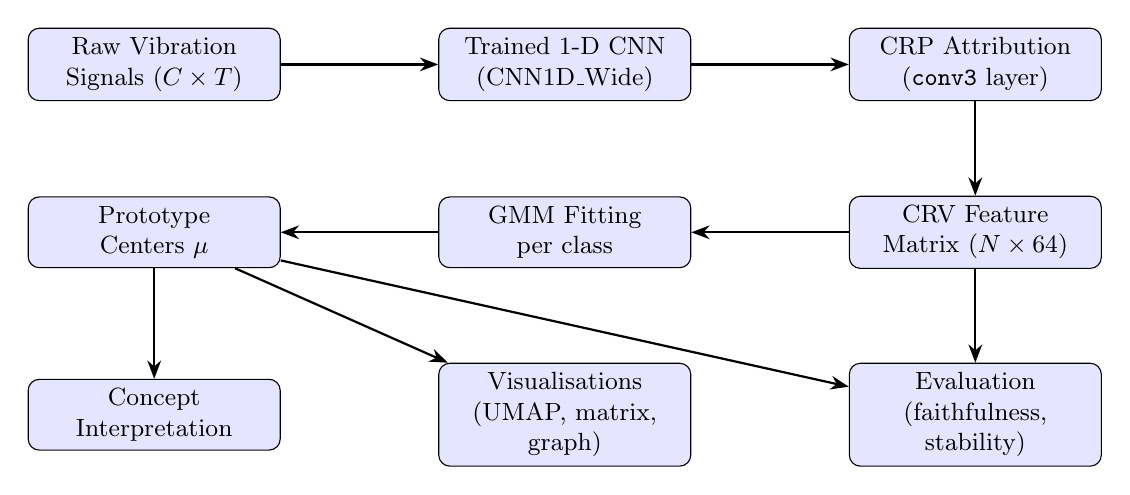
\begin{tikzpicture}[
  node distance=1.2cm and 2.0cm,
  every node/.style={font=\small},
  box/.style={draw, rounded corners, fill=blue!10, minimum width=3.2cm,
              minimum height=0.8cm, align=center},
  decision/.style={draw, diamond, fill=orange!15, aspect=2, align=center,
                   inner sep=2pt},
  arrow/.style={-Stealth, thick},
  label/.style={font=\footnotesize\itshape, text=gray}
]

%% Nodes
\node[box] (data)    {Raw Vibration\\Signals $(C\times T)$};
\node[box, right=of data]  (model)   {Trained 1-D CNN\\(CNN1D\_Wide)};
\node[box, right=of model] (crp)     {CRP Attribution\\(\texttt{conv3} layer)};
\node[box, below=of crp]   (crv)     {CRV Feature\\Matrix $(N\times 64)$};
\node[box, left=of crv]    (gmm)     {GMM Fitting\\per class};
\node[box, left=of gmm]    (proto)   {Prototype\\Centers $\mu$};
\node[box, below=of gmm]   (vis)     {Visualisations\\(UMAP, matrix,\\graph)};
\node[box, right=of vis]   (eval)    {Evaluation\\(faithfulness,\\stability)};
\node[box, left=of vis]    (interp)  {Concept\\Interpretation};

%% Arrows
\draw[arrow] (data)   -- (model);
\draw[arrow] (model)  -- (crp);
\draw[arrow] (crp)    -- (crv);
\draw[arrow] (crv)    -- (gmm);
\draw[arrow] (gmm)    -- (proto);
\draw[arrow] (proto)  -- (vis);
\draw[arrow] (proto)  -- (interp);
\draw[arrow] (crv)    -- (eval);
\draw[arrow] (proto)  -- (eval);

\end{tikzpicture}
\end{center}

%%---------------------------------------------------------------------------
\section{Step-by-Step Description}
%%---------------------------------------------------------------------------

\subsection{Step 1 — CRP Feature Extraction (\texttt{run\_analysis.py})}

For each input sample $\mathbf{x}^{(n)}$ and each predicted class $c$:

\begin{equation}
  \mathrm{CRV}^{(n)} = \bigl[R^{(n)}_{c,1},\; R^{(n)}_{c,2},\; \ldots,\;
                               R^{(n)}_{c,F}\bigr] \in \mathbb{R}^F
\end{equation}

where $R^{(n)}_{c,k}$ is the conditional relevance score of filter $k$ at
layer \texttt{conv3} computed via Concept Relevance Propagation (CRP)~\cite{crp}.
$F=64$ for \texttt{conv3}.

\paragraph{LRP composite.}
The \texttt{CNCValidatedComposite} applies:
\begin{itemize}
  \item \texttt{Epsilon} rule (small $\varepsilon = 0.1$) on fully-connected
        layers and the output layer.
  \item \texttt{ZPlus} rule on all convolutional layers for non-negative
        relevance propagation.
  \item \texttt{Flat} rule on the first convolutional layer to avoid
        attributing relevance to input mean.
\end{itemize}

\subsection{Step 2 — GMM Prototype Discovery (\texttt{discover\_concepts.py})}

The CRV matrix $\mathbf{X}_c \in \mathbb{R}^{N_c \times F}$ for class $c$ is
fitted with a Gaussian Mixture Model:

\begin{equation}
  p(\mathbf{x}) = \sum_{k=1}^{K} \pi_k\,
    \mathcal{N}\!\left(\mathbf{x};\,\boldsymbol{\mu}_k,\,\boldsymbol{\Sigma}_k\right)
\end{equation}

Default settings: $K=3$, diagonal covariance, \texttt{n\_init}=5,
\texttt{max\_iter}=200.

The GMM component means $\{\boldsymbol{\mu}_k\}_{k=1}^K$ serve as
\textbf{prototype centres} and represent prediction sub-strategies.

\subsection{Step 3 — Visualisation}

Three complementary visualisations are generated per class:

\paragraph{(a) UMAP projection (\texttt{plot\_umap\_prototypes}).}
The 64-dimensional CRV space is projected to 2D using UMAP
(\texttt{umap-learn}; PCA fallback if not installed).  Two scatter plots are
produced: one coloured by ground-truth class, one coloured by GMM prototype
assignment.  GMM means $\boldsymbol{\mu}_k$ are projected into the same
embedding and overlaid as stars.

\paragraph{(b) Concept-Prototype Matrix (\texttt{plot\_concept\_prototype\_matrix}).}
Following PCX Figure~5, a matrix $\mathbf{M} \in \mathbb{R}^{T \times K}$ is
formed from the prototype centres:

\begin{equation}
  \mathbf{M}_{i,k} = \mu_k[\mathtt{concept}_i] \times 100
\end{equation}

where the $T$ concept indices are selected as the union of top-$T$ filters by
absolute magnitude across all prototypes, sorted by discriminativeness.  Cells
are colour-coded red (positive) / blue (negative) with text annotation.

\paragraph{(c) Attribution Graph (\texttt{plot\_attribution\_graph}).}
A node-link graph shows the top-$k$ filters (concepts) of a prototype as left
nodes connected to the output class node on the right.  Edge width encodes
$|\mu_k|$; edge colour encodes sign (green = positive, red = negative).

\subsection{Step 4 — Evaluation (\texttt{evaluate\_concepts.py})}

\begin{description}
  \item[Faithfulness] Spearman correlation between filter relevance scores and
        causal intervention effects (suppress filter activations, measure
        prediction change).  PCX target: $\rho > 0.5$.
  \item[Incremental Faithfulness (AUC)] Suppresses filters one at a time in
        relevance order and measures cumulative logit change.  AUC compared to
        random baseline.
  \item[Stability] Mean cosine similarity of CRV vectors within a prototype
        cluster.  PCX target: $> 0.8$.
  \item[Concept Purity] Distinctiveness of prototype clusters (inter-cluster
        distance / intra-cluster distance).
  \item[Coverage] Fraction of samples assigned to each prototype.
\end{description}

%%---------------------------------------------------------------------------
\section{Adaptations from PCX (ImageNet) to TCD (Time-Series)}
%%---------------------------------------------------------------------------

\begin{center}
\begin{tabular}{lll}
\toprule
\textbf{Aspect} & \textbf{PCX (ImageNet)} & \textbf{TCD (vibration)} \\
\midrule
Input & $3\times224\times224$ RGB image & $3\times2000$ vibration signal \\
Concept layer & Last conv (ResNet50) & \texttt{conv3} (64 filters) \\
LRP composite & \texttt{EpsilonPlusFlat} & \texttt{CNCValidatedComposite} \\
Visualisation & Image patches / Grad-CAM & Signal + colour overlay \\
Classes & 1000 ImageNet classes & Binary (OK / NOK) \\
Normalization & \texttt{abs\_norm} per filter & Sum normalization \\
\bottomrule
\end{tabular}
\end{center}

%%---------------------------------------------------------------------------
\section{Known Gaps / Missing Features}
%%---------------------------------------------------------------------------

\begin{center}
\begin{tabular}{lll}
\toprule
\textbf{Feature} & \textbf{PCX} & \textbf{TCD status} \\
\midrule
UMAP of CRV space & \checkmark & \checkmark\ (added) \\
Concept-Prototype Matrix & \checkmark & \checkmark\ (added) \\
Attribution graph & \checkmark & \checkmark\ (wired up) \\
Frequency-domain DFT-LRP & \checkmark & $\times$ (not applicable) \\
\texttt{abs\_norm} normalisation & \checkmark & partial \\
Concept reference images & Image patches & Text labels (Filter~$k$) \\
\bottomrule
\end{tabular}
\end{center}

\subsection{Frequency-Domain DFT-LRP}
PCX for audio uses DFT-based LRP to attribute relevance in the frequency
domain.  For CNC vibration the primary fault signatures are in specific
frequency bands (100--200\,Hz), but DFT-LRP requires a differentiable DFT
layer in the forward pass which is not present in the current CNN1D\_Wide
architecture.  This is a known gap.

\subsection{\texttt{abs\_norm} Normalisation}
PCX normalises each CRV component by the absolute sum across samples
(\texttt{abs\_norm}) to make components comparable across filters with
different activation scales.  TCD currently uses sum normalisation.  Switching
to \texttt{abs\_norm} may improve faithfulness scores.

%%---------------------------------------------------------------------------
\section{Expected Numerical Ranges (from PCX paper)}
%%---------------------------------------------------------------------------

\begin{center}
\begin{tabular}{lll}
\toprule
\textbf{Metric} & \textbf{PCX target} & \textbf{Interpretation} \\
\midrule
Faithfulness (Spearman $\rho$) & $> 0.5$ & Good concept--output alignment \\
Incremental AUC ratio & $> 1.5\times$ random & Relevance ordering is causal \\
Stability (cosine sim.) & $> 0.8$ & Prototype clusters are tight \\
Coverage balance & $1/K \pm 0.1$ & Prototypes cover data uniformly \\
\bottomrule
\end{tabular}
\end{center}

%%---------------------------------------------------------------------------
\section{Configuration Reference}
%%---------------------------------------------------------------------------

The pipeline is controlled by \texttt{configs/default.yaml}.  Key parameters:

\begin{lstlisting}[basicstyle=\ttfamily\small, breaklines=true]
tcd:
  variant: "C"            # Variant C: GMM prototypes in CRP space
  primary_layer: "conv3"  # conv3: 64 filters, richer concept space
  n_prototypes: 3         # GMM components per class
  use_bic_selection: false
  gmm_covariance: "diag"
  gmm_n_init: 5
  gmm_max_iter: 200
\end{lstlisting}

%%---------------------------------------------------------------------------
\begin{thebibliography}{9}
\bibitem{pcx}
  Dreyer, M., et al.\ (2024).
  \emph{Concept-Based Explanations for Graph Neural Networks.}
  NeurIPS 2024.

\bibitem{crp}
  Achtibat, R., et al.\ (2023).
  \emph{From attribution maps to human-interpretable explanations through
  Concept Relevance Propagation.}
  Nature Machine Intelligence, 5, 1006--1019.
\end{thebibliography}

\end{document}
